% Exact representative: F1=(-2,0), F2=(2,0), P=(2,3).
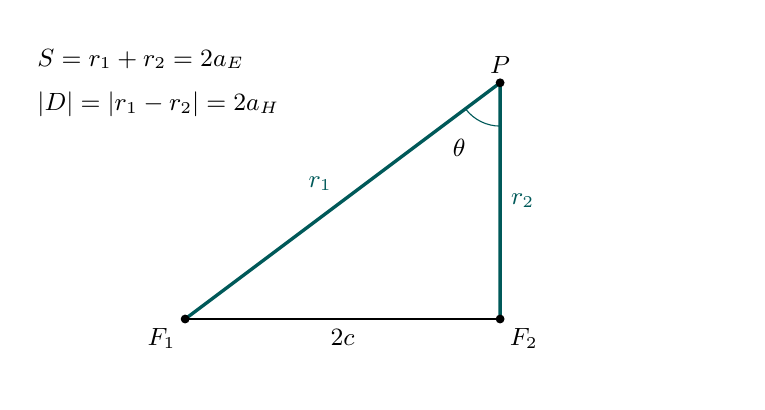
\begin{tikzpicture}[x=1cm,y=1cm,every node/.style={font=\small}]
\path[use as bounding box] (-4,-.8) rectangle (5,3.7);
\coordinate (L) at (-2,0); \coordinate (R) at (2,0); \coordinate (P) at (2,3);
\draw[very thick,teal!70!black] (L)--node[above left] {$r_1$} (P)--node[right] {$r_2$} (R);
\draw[thick] (L)--node[below] {$2c$} (R);
\draw[teal!70!black] (2,2.45) arc(-90:-143.130102:.55);
\node at (1.48,2.18) {$\theta$};
\foreach \v/\lab/\pos in {L/F_1/below left,R/F_2/below right,P/P/above}
  \fill (\v) circle(1.6pt) node[\pos] {$\lab$};
\node[align=left,anchor=west] at (-4,3) {$S=r_1+r_2=2a_E$\\[5pt] $|D|=|r_1-r_2|=2a_H$};
\end{tikzpicture}
